\documentclass[border=10pt]{standalone}
\usepackage[svgnames]{xcolor}
\usepackage{amsmath}
\usepackage{pgfplots}
\pgfplotsset{compat=newest}
\usepackage[sfdefault]{FiraSans}
\usepackage{FiraMono}
\renewcommand*\familydefault{\sfdefault}
\begin{document}
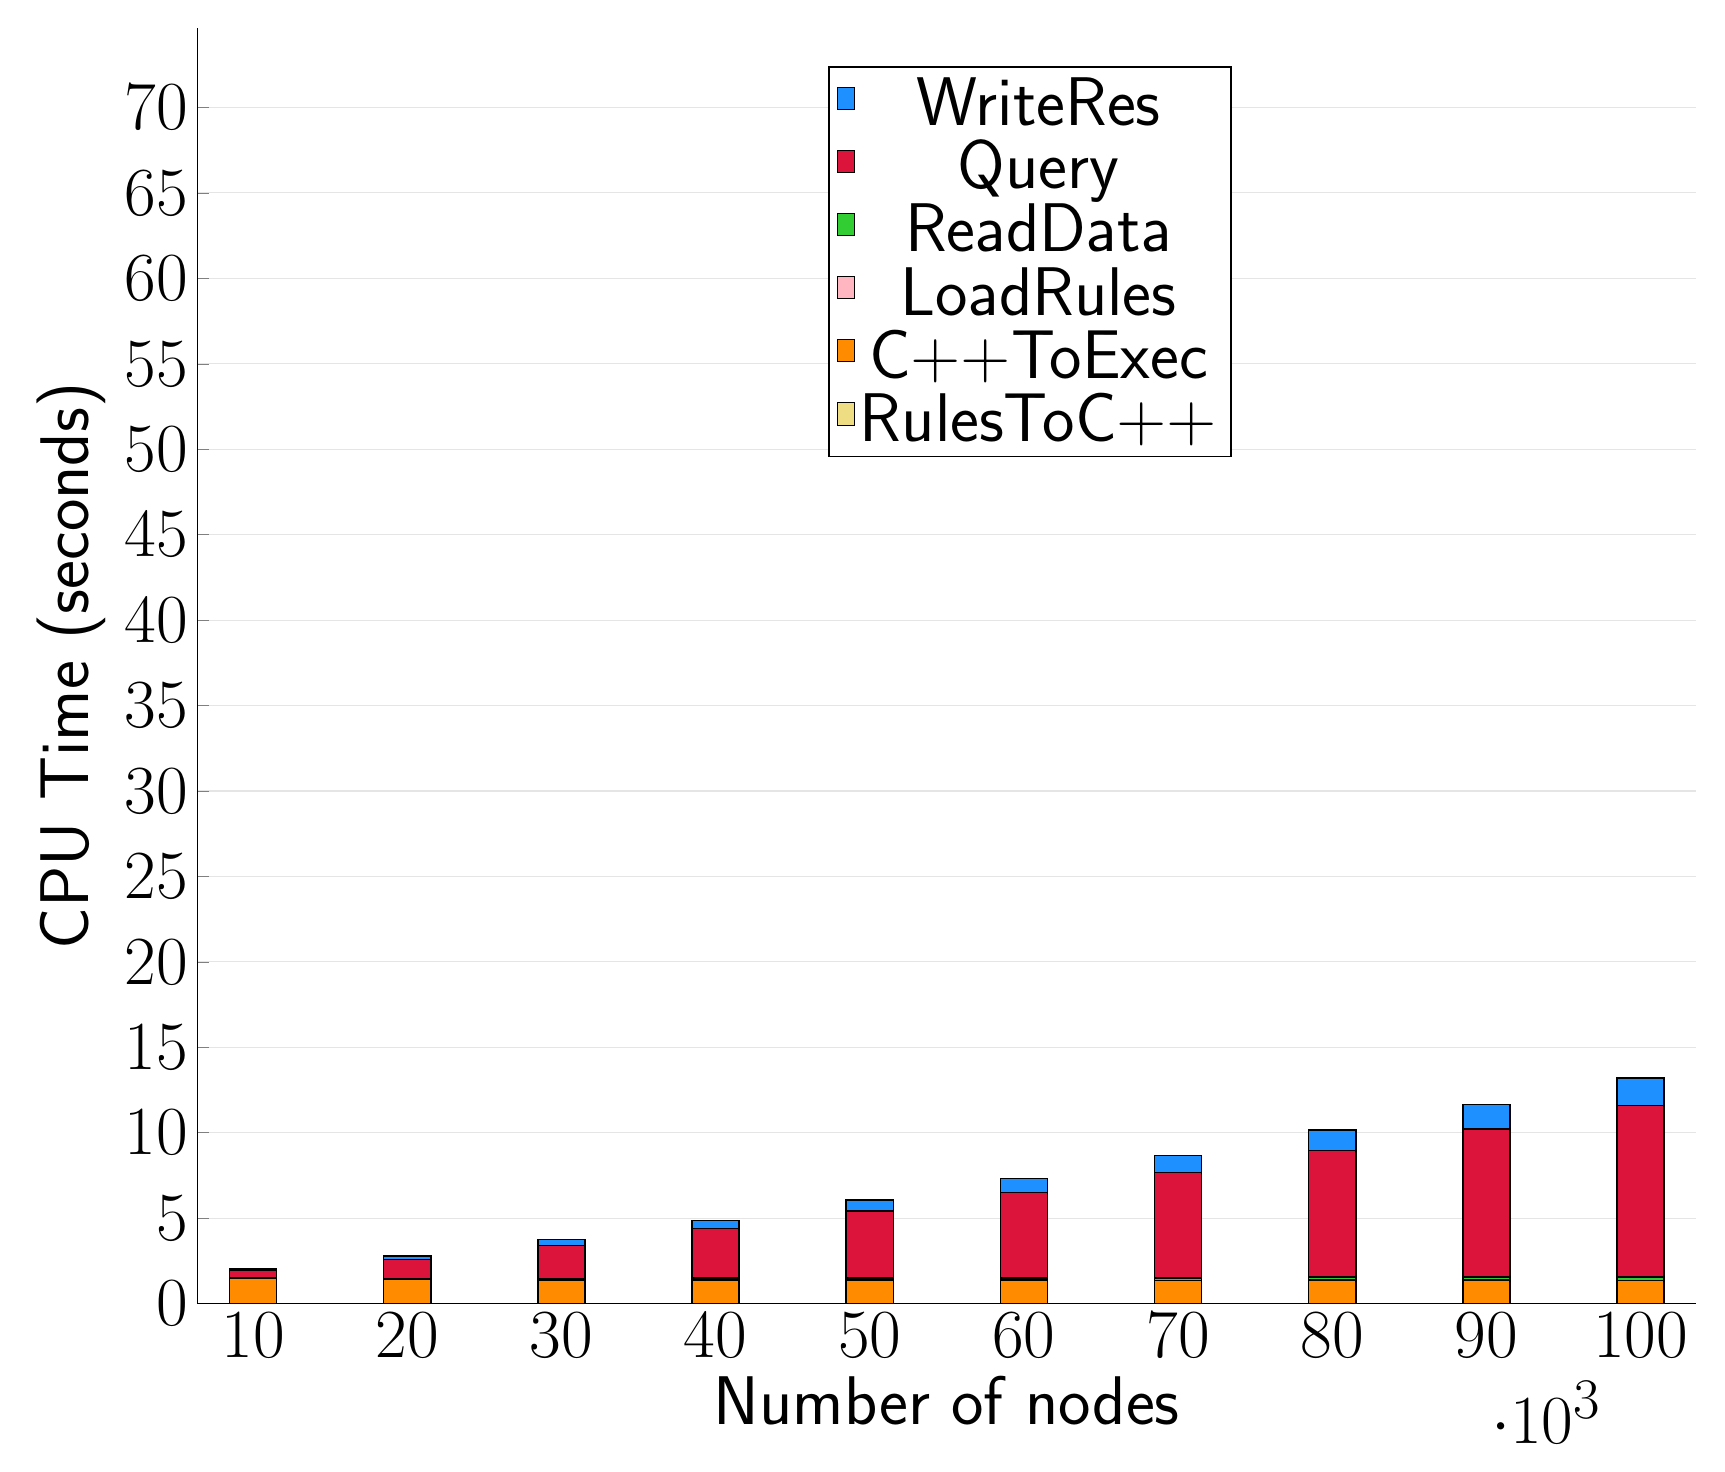
\begin{tikzpicture}
\begin{axis}[
   ybar stacked,
   width=1.7\textwidth,
   bar width=0.6cm,
   ymajorgrids, tick align=inside,
   major grid style={draw=gray!20},
   xtick=data,
   scaled x ticks={base 10:-3},
   ymin=0, ymax=74.64057999999999,
   axis x line*=bottom,
   axis y line*=left,
   enlarge x limits=0.04,
   legend style={
       at={(0.69, 0.97)},
       anchor=north east,
       legend columns=1,
       font=\Huge,
   },
   ylabel={CPU Time (seconds)},
   xlabel={Number of nodes},
   label style={font=\Huge},
   tick label style={font=\Huge},
]
\addlegendimage{fill=DodgerBlue, draw=black, line width=0.2pt}
\addlegendentry{WriteRes}
\addlegendimage{fill=Crimson, draw=black, line width=0.2pt}
\addlegendentry{Query}
\addlegendimage{fill=LimeGreen, draw=black, line width=0.2pt}
\addlegendentry{ReadData}
\addlegendimage{fill=LightPink, draw=black, line width=0.2pt}
\addlegendentry{LoadRules}
\addlegendimage{fill=DarkOrange, draw=black, line width=0.2pt}
\addlegendentry{C++ToExec}
\addlegendimage{fill=LightGoldenrod, draw=black, line width=0.2pt}
\addlegendentry{RulesToC++}
\addplot +[fill=LightGoldenrod, draw=black, line width=0.55pt] coordinates {
(10000, 0.004)
(20000, 0.006000000000000003)
(30000, 0.0)
(40000, 0.0)
(50000, 0.001999999999999999)
(60000, 0.0)
(70000, 0.0)
(80000, 0.0020000000000000018)
(90000, 0.0020000000000000018)
(100000, 0.0)
};
\addplot +[fill=DarkOrange, draw=black, line width=0.55pt] coordinates {
(10000, 1.4580000000000002)
(20000, 1.3980000000000001)
(30000, 1.368)
(40000, 1.3900000000000001)
(50000, 1.3760000000000001)
(60000, 1.366)
(70000, 1.36)
(80000, 1.3760000000000001)
(90000, 1.37)
(100000, 1.358)
};
\addplot +[fill=LightPink, draw=black, line width=0.55pt] coordinates {
(10000, 0.0001684)
(20000, 0.0001226)
(30000, 0.0001222)
(40000, 0.0001692)
(50000, 0.0001466)
(60000, 0.00017280000000000003)
(70000, 0.0001562)
(80000, 0.0001348)
(90000, 0.0001386)
(100000, 0.00015040000000000002)
};
\addplot +[fill=LimeGreen, draw=black, line width=0.55pt] coordinates {
(10000, 0.030203800000000003)
(20000, 0.049249)
(30000, 0.0719254)
(40000, 0.0944756)
(50000, 0.11433940000000001)
(60000, 0.13498459999999998)
(70000, 0.1514872)
(80000, 0.1740026)
(90000, 0.1907146)
(100000, 0.21157120000000001)
};
\addplot +[fill=Crimson, draw=black, line width=0.55pt] coordinates {
(10000, 0.4451904)
(20000, 1.131834)
(30000, 1.970448)
(40000, 2.899878)
(50000, 3.921976)
(60000, 5.012474)
(70000, 6.154302)
(80000, 7.404278)
(90000, 8.667658)
(100000, 10.013678)
};
\addplot +[fill=DodgerBlue, draw=black, line width=0.55pt] coordinates {
(10000, 0.0757984)
(20000, 0.1904204)
(30000, 0.3510922)
(40000, 0.4776344)
(50000, 0.6425826)
(60000, 0.8179632)
(70000, 1.0069624)
(80000, 1.2065540000000001)
(90000, 1.40946)
(100000, 1.6255619999999997)
};
\end{axis}
\end{tikzpicture}

\end{document}
